\section{Networks}
\label{sec:xbrl_networks}

% This section marks the point where the OIM ends and the non-OIM parts of XBRL begin.
% Since XBRL is heavily based on XML, the remainder of this chapter will use XML syntax more heavily.

% Up to now, all concepts in the XBRL taxonomy are treated as independent entities.
% The whole filing can be viewed as an unordered set of facts with no relation between them.
% However, in reality, concepts are not independent of each other.
% Instead, they are related to each other in some way.

% For example, the concepts \texttt{Assets} and \texttt{Liabilities} are related to each other in the sense that they are both part of the concept \texttt{Balance Sheet}.
% Furthermore, the concept \texttt{Assets} can be further divided into the concepts \texttt{Current Assets} and \texttt{Non-Current Assets}.
% The aforementioned relations can be visualized using a directed graph, as shown in figure \ref{fig:example_visualization_network_xbrl}.

% Until this juncture, XBRL taxonomy concepts have been approached as standalone entities,
% presenting the entire filing as a disordered collection of facts without interconnections.
% Contrary to this perspective, concepts are interconnected.

Networks in XBRL are used to represent these relationships between concepts, facts and other elements of an XBRL filing.

For instance, the concepts \texttt{Assets} and \texttt{Liabilities} are interconnected, as both are part to the \texttt{Balance Sheet}.
Moreover, the \texttt{Assets} concept is subdividable into \texttt{Current Assets} and \texttt{Non-Current Assets}.
Such relationships can be depicted through a directed graph, as illustrated in figure \ref{fig:example_visualization_network_xbrl}.

\begin{figure}[H]
    \dirtree{%
        .1 Balance Sheet.
        .2 Assets.
        .3 Current Assets.
        .3 Non-Current Assets.
        .2 Liabilities.
    }
    \caption{Example of relations between concepts in XBRL}
    \label{fig:example_visualization_network_xbrl}
\end{figure}

% A reader with a basic understanding of mathematics will recognize that the above example is a directed acyclic graph (DAG).
% More specifically, the above example is a tree.
% Graphs are commonly used to represent relations between entities.
% In the context of XBRL, graphs are used to represent all kinds of relations between concepts, facts, and other elements of an XBRL filing.
% From now on, I will refer to graphs that represent relations between XBRL elements as \texttt{networks}.

% XBRL commonly uses the term \texttt{Extended Link} or \texttt{Link} to refer to networks or parts of networks.
% I will use the term \texttt{network} throughout this thesis, since it is more intuitive and less ambiguous.
% When I refer to a \texttt{link}, I am referring to something specific in the XBRL specification.
% When I refer to a \texttt{network}, I am referring to the general concept of a network.

% XBRL groups multiple links together into so called \texttt{linkbases}.
% From a semantic perspective, linkbases do not have any meaning.
% From a technical perspective, linkbases are just XML elements that have children that are links. 
A reader with a foundational knowledge of mathematics will identify the aforementioned example as a directed acyclic graph (DAG), 
more specifically, a tree.
Graphs are a widespread method for illustrating relationships among entities.
% Within the XBRL framework, graphs are used to depict the myriad of relationships among concepts, facts, and additional elements of an XBRL filing.
% Therefore, graphs that depict these relationships within XBRL will be referred to as \texttt{networks}.
XBRL often uses the terms \texttt{Extended Link} or \texttt{Link} when discussing networks or their components,
whereas Brel will consistently use the term \texttt{network} to avoid ambiguity.
% For clarity and to avoid ambiguity in this thesis, the term \texttt{network} will be consistently used.
% The term \texttt{link} will denote a specific element within the XBRL specification,
% whereas \texttt{network} will encompass the broader notion of a network.
We exclusively use the term \texttt{Link} to refer to a specific element within the XBRL specification.
XBRL groups multiple links into entities known as \texttt{linkbases}.
% Semantically, linkbases do not convey any inherent meaning.
% Technically, linkbases are XML elements that encapsulate child elements identified as links.

\subsection{Types of Networks}

The XBRL 2.1 specification defines six built in types of networks\cite{xbrl21_terminology}\footnote{The XBRL 2.1 specification is inconsistent about \texttt{link:footnoteLink}. Section 1.4 does not list it as a standard extended link, section 3.5.2.4 does. I will assume that it is a standard extended link.}:

\begin{itemize}
    % \item \texttt{link:presentationLink}: A network that represents the hierarchy of concepts in a report. 
    \item \texttt{link:presentationLink}: This network depicts the hierarchy of concepts.
    % An example of this can be seen in figure \ref{fig:example_visualization_network_xbrl}.
    Figure \ref{fig:example_visualization_network_xbrl} illustrates this such a network.
    % Example: \ref{fig:example_visualization_network_xbrl}.
    \item \texttt{link:calculationLink}: This network shows the calculation relationships between concepts.
    For instance, as shown in Figure \ref{fig:example_visualization_network_xbrl}, 
    \texttt{Assets} results from adding \texttt{Current Assets} to \texttt{Non-Current Assets}.
    % \item \texttt{link:definitionLink}: This network outlines connections beyond those in other networks.
    % The \texttt{definitionLink} is detailed in Section \ref{sec:definitionLink}.
    \item \texttt{link:labelLink}: A network that associates concepts with human-readable labels.
    \item \texttt{link:referenceLink}: This network ties concepts to external references.
    For instance, the concept \texttt{Total Shareholder Return Amount} might have an official definition in the SEC's Code of Federal Regulations (CFR).
    The reference network would link the concept to \texttt{17 CFR 229.402(v)(2)(iv)}\cite{cfr_total_shareholder_return_amount}.
    \item \texttt{link:footnoteLink}: This network associates concepts, facts, and other components with explanatory footnotes.
    \item \texttt{link:definitionLink}: This network outlines relationships that are not covered by other networks.
\end{itemize}

% XBRL refers to these built in networks as \texttt{standard extended links}. 
% If needed, XBRL allows users to define their own networks, which are referred to as \texttt{custom extended links}\cite{xbrl21_terminology}.

% Technically speaking, XBRL does allow networks in XBRL to contain both directed and undirected cycles.
% However, in practice, networks in XBRL are almost always directed acyclic graphs (DAGs).

% In the subsequent sections, I will describe how networks are implemented in XBRL on a conceptual level. 

% Even though labels will be covered in more detail in section \ref{sec:labelLink}, I will already use them throughout this chapter.
% Labels are used to associate report elements with human-readable labels.
% For example, the concept \texttt{us-gaap:CurrentAssets} might have the label "Current Assets" in the English language.
% The main motivation behind this editorial decision is that it makes the chapter easier to read.
XBRL refers to built-in networks as \texttt{standard extended links}.
If necessary, XBRL permits the creation of user-defined networks, known as \texttt{custom extended links}\cite{xbrl21_terminology}.
XBRL does permit both directed and undirected cycles within networks.
Yet, networks within XBRL predominantly take the form of directed acyclic graphs (DAGs).

Although labels will receive a more thorough examination in Section \ref{sec:labelLink}, they will be used throughout this chapter for the sake of readability.
Labels assign human-readable descriptions to concepts. For instance, \texttt{us-gaap:CurrentAssets} may be labeled as "Current Assets" in English.

The following sections will delve into the conceptual implementation of networks within XBRL.

% This approach is adopted to enhance the readability of the chapter.

\subsection{presentationLink}

% The \texttt{link:presentationLink} network is used to represent the hierarchy of concepts in a report.
% I will describe presentationLinks in more detail compared to the other networks, 
% since all other network types are implemented in a similar fashion as presentationLinks.

% XBRL implements all its networks as a list of directed edges called \texttt{arcs}.
% Each arc has a source and a target. Duplicate arcs are not allowed.

% Taking the example from figure \ref{fig:example_visualization_network_xbrl}, the presentationLink network would be represented as the following edge list:
The \texttt{link:presentationLink} network represents concept hierarchies within a report.
I will offer a more detailed exploration of presentationLinks compared to other network types,
as the implementation of all other network types mirrors that of presentationLinks.

XBRL structures its networks through a sequence of directed edges, referred to as \texttt{arcs}.
Each arc possesses a source and a target, with duplicate arcs being prohibited.
Referring to the illustration in figure \ref{fig:example_visualization_network_xbrl},
the presentationLink network would manifest as the following list of edges:

% don't use the minted package
\begin{figure}[H]
    \begin{verbatim}
        Balance Sheet -> Assets
        Assets -> Current Assets
        Assets -> Non-Current Assets
        Balance Sheet -> Liabilities
    \end{verbatim}
    \caption{Example of a presentationLink network in edge list format}
    \label{fig:example_visualization_network_xbrl_edge_list}
\end{figure}

% Each arc in the example \ref{fig:example_visualization_network_xbrl_edge_list} is represented as a \texttt{link:presentationArc} element in XBRL.
% Besides presentationArcs, presentationLinks contain so called "locators" \texttt{link:loc} that represent the nodes in the network.
% In case of a presentation network, the locators are references to the concepts in the XBRL taxonomy. 
% In other networks, locators can be references to other elements, such as facts.

% Going back to the example in figure \ref{fig:example_visualization_network_xbrl_edge_list}, 
% the first arc \texttt{Balance Sheet -> Assets} would be represented as follows in XML syntax:
In Figure \ref{fig:example_visualization_network_xbrl_edge_list}, every arc is denoted by a \texttt{link:presentationArc} element within XBRL.
PresentationLinks, in addition to presentationArcs, include "locators" indicating network nodes.
For presentation networks, locators point to XBRL taxonomy concepts.
% Locators in other networks may refer to different elements, like facts.
Referring to the example in Figure \ref{fig:example_visualization_network_xbrl_edge_list},
the arc from \texttt{Balance Sheet} to \texttt{Assets} is represented in XML as follows:

\begin{figure}[H]
    \centering
    \begin{lstlisting}[language=XML, basicstyle=\small\ttfamily]
<link:loc 
    xlink:type="locator" 
    xlink:href="file_1.xsd#BalanceSheet"
    xlink:label="BalanceSheet_loc"
/>
<link:loc 
    xlink:type="locator" 
    xlink:href="file_1.xsd#Assets"
    xlink:label="Assets_loc"
/>
<link:presentationArc 
    xlink:type="arc" 
    xlink:arcrole="http://www.xbrl.org/2003/arcrole/parent-child" 
    xlink:from="BalanceSheet_loc" 
    xlink:to="Assets_loc"
    order="1"
/>
\end{lstlisting}
    \caption{Example of a presentationArc in XML syntax}
    \label{fig:example_presentation_arc_xml}
\end{figure}

% The XML snippet in figure \ref{fig:example_presentation_arc_xml} contains two locators and one arc.
% The two locators represent the nodes of the arc, referencing the concepts \texttt{BalanceSheet} and \texttt{Assets} respectively.
% The arc represents the edge between the two nodes.

% Let us look at the XML snippet \ref{fig:example_presentation_arc_xml} step by step.

% \begin{itemize}
%     \item \textbf{Type}: The \texttt{xlink:type} attribute specifies the types for both the locators and the arc.
%     For the former, the type is \texttt{locator}, whereas for the latter, the type is \texttt{arc}.
%     \item \textbf{Connect nodes and edges}: Both locators contain an \texttt{xlink:label} attribute that uniquely identifies the locator.
%     The arc links the two locators together using the \texttt{xlink:from} and \texttt{xlink:to} attributes.
%     \item \textbf{Edge order}: The outgoing edges of a node are ordered using the \texttt{order} attribute of the arc.
%     \item \textbf{Arcrole}: The \texttt{xlink:arcrole} attribute of the arc specifies the kind of relation between the source and the target of the arc.
%     In case of a presentationLink, the \texttt{xlink:arcrole} attribute is always set to \texttt{parent-child}.\label{sec:arcrole}
% \end{itemize}

% Locators and arcs form the basic building blocks of all networks in XBRL, notably presentationLinks.
% A presentationLink is just a container for locators and arcs.
% To build a fully featured presentation network such as in figure \ref{fig:example_visualization_network_xbrl},
% we need to add more locators and arcs to the presentationLink.
% To avoid cluttering the chapter with XML snippets, I will only describe the XML syntax for the first arc in the network.

The XML snippet in Figure \ref{fig:example_presentation_arc_xml} displays two locators and one arc, where the locators represent the nodes linked by the arc, corresponding to the \texttt{BalanceSheet} and \texttt{Assets} concepts.
The arc signifies the connection between these two nodes.

The breakdown of the XML snippet \ref{fig:example_presentation_arc_xml} is as follows:

\begin{itemize}
    \item \textbf{Type}: The attribute \texttt{xlink:type} defines the roles of locators and the arc, labeling locators as \texttt{locator} and the arc as \texttt{arc}.
    \item \textbf{Connecting nodes to edges}: Each locator has a \texttt{xlink:label} attribute for identification, while the arc uses \texttt{xlink:from} and \texttt{xlink:to} attributes to connect the locators.
    \item \textbf{Ordering edges}: The \texttt{order} attribute on the arc dictates the sequence of outgoing edges from a node.
    \item \textbf{Arcrole}: The arc's \texttt{xlink:arcrole} attribute clarifies the relationship between the arc's source and target, set to \texttt{parent-child} for presentationLinks.
\end{itemize}

In XBRL, locators and arcs are fundamental to constructing networks, especially presentationLinks.
For brevity, only the XML syntax for the first arc in the network is provided.
% Additional arcs and locators are defined in a similar manner.
A presentationLink is merely a collection of locators and arcs.
To craft a comprehensive presentation network like the one in figure \ref{fig:example_visualization_network_xbrl}, additional locators and arcs are incorporated into the presentationLink.
% For brevity, further XML syntax details will be limited to the first arc in the network.


% The \texttt{xlink:from} attribute of the \texttt{link:presentationArc} element references the \texttt{xlink:label} attribute of the \texttt{link:loc} element that represents the source of the arc.
% The same applies to the \texttt{xlink:to} attribute of the \texttt{link:presentationArc} element.

% Both locators contain a \texttt{xlink:href} attribute that references the concept in the XBRL taxonomy that the locator represents.
% This reference can even point to a different file, as shown in figure \ref{fig:example_presentation_arc_xml}.

% The \texttt{xlink:type} on the elements helps the XML parser to determine the type of the element.
% Note that the XML tag \texttt{link:presentationArc} already hints at the fact that this element is a type of arc.
% However, the \texttt{xlink:type} attribute is still required and provides parsers with a more reliable way to determine if an element is an arc, a locator, or something else. 

% The \texttt{order} attribute of the \texttt{link:presentationArc} element specifies in which order the children of the source of the arc should be displayed.


% \section{Arcroles}
% \label{sec:arcrole}
% The \texttt{xlink:arcrole} attribute of the \texttt{link:presentationArc} element specifies the kind of relation between the source and the target of the arc.
% % In case of a presentationLink, the \texttt{xlink:arcrole} attribute is always set to \texttt{parent-child}.
% Even though presentationLinks only allow the \texttt{parent-child} arcrole, other networks allow different arcroles.
% % For different networks, the \texttt{xlink:arcrole} attribute can be set to different values.
% It can even be set to different values for different arcs in the same network.

% XBRL packages the set of arcs and locators into a \texttt{link:presentationLink} element.
% This element contains a \texttt{xlink:role} attribute that specifies the role of the presentationLink.
% Roles are a more advanced concept that I will introduce in section \ref{sec:roles}.
% For now, think of the \texttt{link:presentationLink} element as a container for the arcs and locators.

\subsection{Motivation for Report Elements}
\label{sec:report_elements_motivation}

% Up to this point, I have only described how presentation networks are implemented in XBRL.
% I also mentioned that presentation networks introduce a hierarchy of concepts, but this is not entirely true.

% I have introduced concepts as the "what"-part of a fact. 
% For example, if the company Foo reports a revenue of 1000 USD in 2019, the concept \texttt{Revenue} is the "what"-part of the fact.

% However, if we look at the presentation network in figure \ref{fig:example_visualization_network_xbrl}, not all of the elements in the network can have a fact associated with them.
% An example of this is the concept \texttt{BalanceSheet}.
% In XBRL, concepts that can not have a fact associated with them are called \texttt{Abstract}.

% XBRL combines abstracts and concepts under the umbrella term "report element".
% Report elements are, as the name suggests, elements that can appear in a report.
% Some of these report elements are used for facts, namely the concepts.
% Others are used to represent the structure of the report, namely the abstracts.
% There are six types of report elements in total\cite{oim}. 
% I will introduce them as they come up in the subsequent sections.

% With the introduction of report elements, our notion of a presentation network changes slightly.
% Instead of introducing a hierarchy of concepts, presentation networks introduce a hierarchy of report elements.
% However, our notion of a fact stays the same.
% A fact is still requires a concept, not a report element.
Until now, the focus has been on the implementation of presentation networks in XBRL and their role in structuring a hierarchy of concepts. 
However, this explanation is not completely accurate.

Concepts have been defined as the "what" aspect of a fact. For instance, when the company Foo declares a revenue of 1000 USD for the year 2019, 
the "what" part is represented by the concept \texttt{Revenue}.

Yet, not every element within the presentation network, as seen in figure \ref{fig:example_visualization_network_xbrl}, is capable of being linked to a fact. 
The \texttt{BalanceSheet} concept serves as an example. 
In XBRL terminology, concepts that cannot be directly associated with facts are termed \texttt{Abstract}.

XBRL categorizes both abstracts and concepts under the collective term "report element". 
These elements can appear within a report, with concepts being directly linked to facts and abstracts outlining the report's structure. 
In total, XBRL recognizes six types of report elements, which will be detailed in subsequent sections.

With the clarification of report elements, the understanding of presentation networks slightly shifts. 
Instead of merely organizing concepts, presentation networks arrange report elements into a hierarchy. 
% Nonetheless, the concept of a fact remains unchanged, necessitating a concept, not just any report element.
Nonetheless, within the context of a fact, a concept is still required, not just any report element. 

\subsection{calculationLink}
\label{sec:calculationLink}

% The \texttt{link:calculationLink} network is used to represent how concepts are calculated from other concepts.
% More specifically, it is used to represent how a concept is the sum of other concepts.
% Under the hood, calculationLinks are implemented in the same way as presentationLinks, but there are a few differences:

% \begin{enumerate}
%     \item Arcs are now called \texttt{link:calculationArc}.
%     \item Links are \texttt{link:calculationLink}.
%     \item The \texttt{xlink:arcrole} attribute of the \texttt{link:calculationArc} element is set to \texttt{summation-item}.
%     \item The \texttt{link:calculationArc} element has an additional attribute called \texttt{weight}.
%     \item All locators in the link are references to concepts, not just report elements.
% \end{enumerate}

% Most of these differences are self-explanatory and do not have any semantic implications.
% However, the last two differences are worth explaining in more detail.

The \texttt{link:calculationLink} network delineates how concepts derive from the sum of other concepts.  
Although built similarly to presentationLinks, calculationLinks exhibit notable differences:  

\begin{enumerate}  
    \item Arcs are termed \texttt{link:calculationArc}.  
    \item Links are designated as \texttt{link:calculationLink}.  
    \item The \texttt{xlink:arcrole} attribute for \texttt{link:calculationArc} is set to \texttt{summation-item}.  
    \item An extra attribute, \texttt{weight}, is part of the \texttt{link:calculationArc}.  
    \item All locators within the link refer exclusively to concepts.  
\end{enumerate}  

% While the initial distinctions are direct and bear no semantic impact, 
While the first three distinctions bear no semantic impact,  
the addition of the \texttt{weight} attribute and the locator's exclusive reference to concepts are pivotal aspects that warrant further explanation.

% The main motivation behind calculation networks is so that XBRL processors can either calculate the value of a concept or check if the value of a concept is computed correctly and consistently.
% In the case of our XBRL processor Brel, the main focus is on the latter. 
% Chapter 6.4 of "The XBRL Book" \cite{fourny2023xbrl} describes the different consistency checks in more detail.

% Facts that have a concept within a calculation network are computed as a weighted sum of their children.
% The \texttt{weight} attribute of the \texttt{link:calculationArc} element specifies the weight of the child in the sum.
% Additionally, facts can only be associated with concepts, not just any report element.
% Therefore, all locators in a calculation network are references to concepts.

% In the section on concepts \ref{sec:concepts}, I have introduced the \texttt{balance} aspect of a concept.
% It specifies if the concept is a debit or a credit.
% The XBRL 2.1 specification enforces some constraints on the \texttt{balance} aspect of concepts in combination with the \texttt{weight} attribute of the \texttt{link:calculationArc} element \cite{xbrl21_concept}.
% If one concept has a \texttt{balance} of \texttt{debit} and another concept has a \texttt{balance} of \texttt{credit}, then their connecting arc must have a negative \texttt{weight}.
% If both concepts have the same \texttt{balance}, then their connecting arc must have a positive \texttt{weight}.
Calculation networks in XBRL are designed to enable processors to calculate or verify the correctness and consistency of a fact's value.  
For the XBRL processor Brel, the emphasis is on verification.  
"The XBRL Book" delves into various consistency checks in Chapter 6.4 \cite{fourny2023xbrl}.  

In calculation networks, facts linked to a concept are calculated as the weighted sum of their child concepts.  
The \texttt{weight} attribute in the \texttt{link:calculationArc} element determines the child's contribution to this sum.  
Moreover, facts are associated exclusively with concepts, not any report element,  
hence all locators in a calculation network reference concepts.  

The concept's \texttt{balance} attribute, introduced in Section \ref{sec:concepts}, indicates whether it is a debit or credit.  
XBRL 2.1 specification imposes rules on the interaction between a concept's \texttt{balance} attribute and the \texttt{weight} attribute of a \texttt{link:calculationArc} \cite{xbrl21_concept}.  
A negative \texttt{weight} is required if one concept is a debit and the other is a credit.  
Conversely, a positive \texttt{weight} is necessary if both concepts share the same \texttt{balance}.

% small table describing the balance and weight constraints
\begin{figure}[H]
    \label{fig:balance_weight_constraints}
    \centering
    \begin{tabular}{|l|l|l|}
        \hline
        \textbf{Concept 1} & \textbf{Concept 2} & \textbf{Connecting edge weight} \\ \hline
        Debit              & Credit             & $\leq 0$        \\ \hline
        Credit             & Debit              & $\leq 0$        \\ \hline
        Debit              & Debit              & $\geq 0$        \\ \hline
        Credit             & Credit             & $\geq 0$        \\ \hline
    \end{tabular}
    \caption{Balance and weight constraints in calculation networks}
\end{figure}

% A network that is consistent with the balance and weight constraints is called a \texttt{balance consistent network}.\cite{fourny2023xbrl}

% \label{sec:roll_up_consistency}
% Balance consistency is not the only kind of consistency that calculation networks can be checked for.
% Another kind of consistency is \texttt{roll-up consistency} which comes in two flavors: \texttt{simple roll-up consistency} and \texttt{nested roll-up consistency}. 

% Simple roll-up is roll-up consistency without any nested concepts. 
% So the calculation network can only have a depth of 1.

% Nested roll-up consistency is roll-up consistency with nested concepts.
% So the calculation network can have a depth of more than 1.

% \texttt{Roll-up consistency} requires a calculation network as well as a presentation network and checks if the structure of the two networks is consistent.
% For example, if the calculation network contains the arc \texttt{Assets -> Savings Accounts}, 
% then the presentation network must also contain the arc \texttt{Assets [Abstract] -> Savings Accounts}.

% Remember that calculation networks can only contain concepts, not abstracts. 
% So the report element \texttt{Assets} in the calculation network and the report element \texttt{Assets [Abstract]} in the presentation network are not the same.
% But how does XBRL know that they are related?

% The answer is that the two report elements are related by the presentation network.
% It contains the arc \texttt{Assets [Abstract] -> Assets}.

% Let us visualize this example in figure \ref{fig:example_roll_up_consistency}, 
% which shows the calculation network and the presentation network side by side.
% The two networks are roll-up consistent with each other.
% The example is expanded a bit and also contains the concepts \texttt{UBS Savings Account}, 
% \texttt{Raiffeisen Savings Account} and \texttt{Liabilities}.
% Note that the calculation network contains weights for the arcs, but the presentation network does not.
A network that adheres to the specified balance and weight rules is recognized as a \texttt{balance consistent network} \cite{fourny2023xbrl}.

\label{sec:roll_up_consistency}  
Balance consistency represents just one form of consistency applicable to calculation networks.  
Another form is \texttt{roll-up consistency}, which is categorized into: \texttt{simple roll-up consistency} and \texttt{nested roll-up consistency}.  

\begin{itemize}
    \item \texttt{Simple roll-up consistency} pertains to networks without nested concepts, limiting the network to a depth of 1.  
    \item \texttt{Nested roll-up consistency} involves networks with nested concepts, allowing for a network depth greater than 1.
\end{itemize}

% \texttt{Simple roll-up consistency} pertains to networks without nested concepts, limiting the network to a depth of 1.  

% \texttt{Nested roll-up consistency} involves networks with nested concepts, allowing for a network depth greater than 1.  

\texttt{Roll-up consistency} examines both calculation and presentation networks to ensure their structures align.  
For instance, if a calculation network includes the arc \texttt{Assets -> Savings Accounts},  
the presentation network must also feature the arc \texttt{Assets [Abstract] -> Savings Accounts}.  

% The concept us-gaap:Revenue can be divided into us-gaap:Sales, us-gaap:Intrest and us-gaap:OtherRevenue.

It's important to note that calculation networks consist solely of concepts, excluding abstracts.  
Thus, the report element \texttt{Assets} in the calculation network differs from \texttt{Assets [Abstract]} in the presentation network.  
The relationship between these two elements is established through the presentation network, which includes the arc \texttt{Assets [Abstract] -> Assets}.  

Figure \ref{fig:example_roll_up_consistency} will illustrate this concept by displaying the calculation and presentation networks side by side,  
demonstrating their roll-up consistency.  
The example is further detailed with concepts such as \texttt{UBS Savings Account}, \texttt{Raiffeisen Savings Account}, and \texttt{Liabilities}.  
Note, the calculation network includes arc weights, unlike the presentation network.

\begin{figure}[H]
    \caption{Example of nested roll-up consistency}
    \label{fig:example_roll_up_consistency}
    % draw the calculation- and presentation network side by side
    \begin{minipage}{0.8\textwidth}
        \dirtree{%
            .1 Assets (weight: 1).
            .2 Savings Accounts (weight: 1).
            .3 UBS Savings Account (weight: 1).
            .3 Raiffeisen Savings Account (weight: 1).
            .2 Liabilities (weight: -1).
        }
        \caption{Calculation network}
        \label{fig:example_roll_up_consistency_calculation}
    \end{minipage}
    \begin{minipage}{0.8\textwidth}
        \dirtree{%
            .1 Assets [Abstract].
            .2 Savings Accounts [Abstract].
            .3 UBS Savings Account.
            .3 Raiffeisen Savings Account.
            .3 Savings Accounts.
            .2 Assets.
            .2 Liabilities.
        }
        \caption{Presentation network}
        \label{fig:example_roll_up_consistency_presentation}
    \end{minipage}
\end{figure}

% The presentation network in figure \ref{fig:example_roll_up_consistency} is roll-up consistent with the calculation network.
% It contains the two abstracts \texttt{Assets [Abstract]} and \texttt{Savings Accounts [Abstract]}, 
% which are not present in the calculation network. 
% They take the role of the concepts \texttt{Assets} and \texttt{Savings Accounts} in the calculation network.

% Besides roll-up and balance consistency, there is a third kind of consistency. 
% XBRL does not have a name for it, but I will refer to it as \texttt{aggregation consistency}.
% It checks if in a calculation network, for each concept, the child concepts add up to their parent concept.
% Going back to our example in figure \ref{fig:example_roll_up_consistency},
% the values of the UBS Savings Account and the Raiffeisen Savings Account should add up to the value of the Savings Accounts concept.
% Aggregation consistency uses weighted sums to add up the values of the child concepts, 
% where the weight of a child concept is the weight of the connecting arc.

% To check for aggregation consistency, we need to know the values of the facts that are associated with the concepts.
% So aggregation consistency checks a list of facts against a calculation network.

% Aggregation consistency is best explained using an example.
% Consider the following list of facts \ref{fig:example_facts_aggregation_consistency} for the calculation network in figure \ref{fig:example_roll_up_consistency}:
In Figure \ref{fig:example_roll_up_consistency}, the presentation network is roll-up consistent with the calculation network.  
It includes two abstracts, \texttt{Assets [Abstract]} and \texttt{Savings Accounts [Abstract]}, which do not appear in the calculation network.  
These abstracts act as placeholders for the concepts \texttt{Assets} and \texttt{Savings Accounts} in the calculation network.

% Beyond roll-up and balance consistency, there exists a third form of consistency, unnamed by XBRL, which I will term \texttt{aggregation consistency}.  
% This type of consistency ensures that within a calculation network, the sum of child concepts accurately contributes to the value of their parent concept.  
Beyond roll-up and balance consistency, calculation networks should ensure that the sum of child concept's facts accurately contributes to the value of their parent concept's fact.
We will refer to this as \texttt{aggregation consistency}.
Referring to our example in Figure \ref{fig:example_roll_up_consistency},  
the values for \texttt{UBS Savings Account} and \texttt{Raiffeisen Savings Account} should aggregate to match the \texttt{Savings Accounts} concept's total value.  
Aggregation consistency relies on the weighted sums of child concepts, with each weight determined by the arc's weight.

For aggregation consistency evaluation, it's essential to have the values of facts linked to the concepts,  
implying that this form of consistency compares a list of facts against a calculation network.

A practical demonstration of aggregation consistency can be seen in the list of facts presented in Figure \ref{fig:example_facts_aggregation_consistency}, 
relevant to the calculation network in Figure \ref{fig:example_roll_up_consistency_calculation}:

% \begin{figure}[H]
%     \caption{List of facts for the calculation network in figure \ref{fig:example_roll_up_consistency}}
%     \label{fig:example_facts}
%     \begin{tabular}{|r|r|r|r|l|}
%         \hline
%         \textbf{Concept} & \textbf{Entity} & \textbf{Period} & \textbf{Unit} & \textbf{Value} \\ \hline
%         UBS Savings Account & Alice & 2019 & USD & 1000 \\ \hline
%         Raiffeisen Savings Account & Alice & 2019 & USD & 2000 \\ \hline
%         Savings Accounts & Alice & 2019 & USD & 3000 \\ \hline
%         Liability & Alice & 2019 & USD & 500 \\ \hline
%         Assets & Alice & 2019 & USD & 2500 \\ \hline
%         UBs Savings Account & Alice & 2020 & USD & 2000 \\ \hline
%         Raiffeisen Savings Account & Alice & 2020 & USD & 3000 \\ \hline
%         Savings Accounts & Alice & 2020 & USD & 5000 \\ \hline
%         Liability & Alice & 2020 & USD & 1000 \\ \hline
%         Assets & Alice & 2020 & USD & 3999 \\ \hline
%     \end{tabular}
% \end{figure}

\begin{figure}[H]
    \caption{Alice's savings accounts and liabilities in CHF}
    \label{fig:example_facts_aggregation_consistency}
    \centering 
    \begin{tabular}{|r|r|r|}
        \hline
        \textbf{Concept} & \textbf{2022} & \textbf{2023} \\ \hline
        UBS Savings Account & 1000 & 1000 \\ \hline
        Raiffeisen Savings Account & 2000 & 3000 \\ \hline
        Savings Accounts & 3000 & 4000 \\ \hline
        Liability & 500 & 500 \\ \hline
        Assets & 2500 & 3499 \\ \hline
    \end{tabular}
\end{figure}

% As you can see, there are two facts reported against each concept, one for 2022 and one for 2023.

% If there are multiple facts reported against a concept, then we iterate over them and "pin" all aspects except for the concept.
% Next, we go to the list of all facts and filter out all facts that have the same pinned aspects.
% Finally, we check for aggregation consistency using the filtered list of facts and the calculation network.

% In our example, we would first check all facts for 2022, then all facts for 2023.
% The list of facts is aggregation consistent for the year 2022, since the values of the UBS Savings Account and the Raiffeisen Savings Account add up to the value of the Savings Accounts concept.
% Also, the value of the Savings Accounts minus the value of the Liabilities concept adds up to the value of the Assets concept.

% However, the list of facts is not aggregation consistent for the year 2023.
% The reason being that the value of the Savings Accounts minus the value of the Liabilities concept does not result in the value of the Assets concept.

As demonstrated, each concept has two reported facts, one for 2022 and another for 2023.

When multiple facts are reported for a concept, the process involves iterating through these facts and "pinning" all aspects except for the concept itself.  
Subsequently, a search through all facts is conducted to identify those with identical pinned aspects.  
Using this refined list of facts and the calculation network, aggregation consistency is then assessed.

In the given example, the assessment would commence with all facts for 2022, followed by those for 2023.  
For 2022, the list of facts is deemed aggregation consistent as the sums of the UBS Savings Account and the Raiffeisen Savings Account align with the total value of the Savings Accounts concept.  
Additionally, subtracting the value of the Liabilities concept from the Savings Accounts concept yields the value of the Assets concept, affirming consistency.

However, for the year 2023, the facts list does not maintain aggregation consistency.  
The discrepancy arises because the combined value of the Savings Accounts, after adjusting for the Liabilities concept's value, fails to match the declared value of the Assets concept.

\subsection{definitionLink}
\label{sec:definitionLink}

% The \texttt{link:definitionLink} network is used to represent the other relations between report elements.
% From an implementation perspective, definitionLinks function in the same way as presentationLinks and calculationLinks.
% The only syntactic differences are the following:

% \begin{enumerate}
%     \item The arcs are called \texttt{link:definitionArc}
%     \item The link is called \texttt{link:definitionLink}
%     \item The \texttt{xlink:arcrole} attribute of the \texttt{link:definitionArc} can be a myriad of different values, even within the same network.
% \end{enumerate}

% Both the link- and the arc-names are self-explanatory and do not have any semantic implications.
% The \texttt{xlink:arcrole} attributes describe the different relations between the source and the target of the arc.

% For instance \texttt{essence-alias} is used to represent that one report element is an alias for another report element.
% \texttt{hypercube-dimension} represents that a "dimension" report element is a member of a "hypercube" report element.
% Both hypercubes and dimensions will be covered in more detail in section \ref{sec:hypercubes}.

% Definition networks may contain more than just the two aforementioned arc roles.
% The purpose of a \texttt{link:definitionLink} is to capture the relationships not covered by the other networks.
% Among other things, it contains important information for identifying the type of a report element.
% Hypercubes, which will be covered in more detail in section \ref{sec:hypercubes}, make extensive use of definition networks.

The \texttt{link:definitionLink} network represents various relationships between report elements not encapsulated by presentation or calculation networks.  
In terms of implementation, definitionLinks operate similarly to presentationLinks and calculationLinks,  
with a few syntactic distinctions:

\begin{enumerate}  
    \item Arcs are denoted as \texttt{link:definitionArc}  
    \item The network itself is referred to as \texttt{link:definitionLink}  
    \item The \texttt{xlink:arcrole} attribute for \texttt{link:definitionArc} encompasses a range of values, varying within and across networks. 
\end{enumerate}  

The naming conventions for links and arcs are straightforward and carry no inherent semantic significance.  
The \texttt{xlink:arcrole} attribute specifies the nature of the relationships between arc sources and targets.  

For example, the \texttt{essence-alias} arcrole indicates that one report element serves as an alias for another,  
while \texttt{hypercube-dimension} signifies the association of a "dimension" report element with a "hypercube" report element.  
Further details on hypercubes and dimensions will be explored in Section \ref{sec:hypercubes}.  

Definition networks extend beyond these two arc roles, aiming to document relationships unaddressed by other network types.  
They are instrumental in clarifying the classification of report elements,  
with hypercubes, discussed further in Section \ref{sec:hypercubes}, relying heavily on definition networks.

\subsection{labelLink}
\label{sec:labelLink}

% The \texttt{link:labelLink} network is used to associate report elements with human-readable labels.
% Thus far, we referred to report elements using their QName.
% Obviously, if we were to open an XBRL report in a viewer such as Arelle, we would not be greeted with QNames for the concepts, abstracts, etc.
% Instead, we would see nicely formatted human-readable labels.

% The following figure shows an example of the condensed consolidated statement of income of the Coca Cola Company\cite{ko2019q2} of Q2 2019 as displayed in Arelle\cite{arelle}.

The \texttt{link:labelLink} network serves to connect report elements with labels that are readable and understandable by humans.
Instead of presenting users with the QName of report elements, applications like Arelle display human-readable labels.

For example, in the Coca-Cola Company's condensed consolidated statement of income for Q2 2019\cite{ko2019q2},
the concept identified as \texttt{us-gaap:Revenues} is shown in Arelle as "Net Operating Revenues",
thanks to the \texttt{link:labelLink} network included in the XBRL report.

\begin{figure}[H]
    \centering
    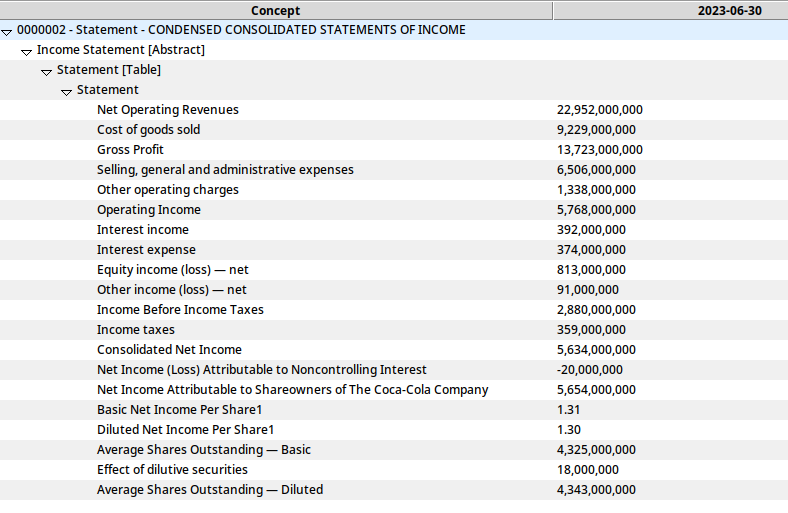
\includegraphics[width=\textwidth]{images/coca_cola_2019_q2.png}
    \caption{Statement of income of the Coca-Cola Company of Q2 2019}
    \label{fig:coca_cola_2019_q2}
\end{figure}

% Let us take a closer look at the first concept of the statement of income: Revenue.
% Even though the concept for the revenue is \texttt{us-gaap:Revenues}, Arelle displays it as "Net Operating Revenues".

% Arelle achieves this by using the \texttt{link:labelLink} network that is part of the XBRL report. 
% LabelLinks are another type of extended link that associates report elements with strings.
% They are implemented in the same way as presentationLinks and calculationLinks, but this time they not only contain arcs and locators, but also \texttt{link:label} elements.

% From a semantic perspective, labels are different from report elements such as concepts and abstracts.
% Instead, they are a kind of \texttt{resource}.
% Resources are essentially metadata about report elements, facts, and other elements of an XBRL report.

% The approach that XBRL takes to labels and other resources is quite interesting.
% Going back to our example in figure \ref{fig:coca_cola_2019_q2}, the definition of the concept \texttt{us-gaap:Revenues} happens independently from any labels that are associated with it.
% The labels are later associated with the concept using the \texttt{link:labelLink} network.
% In fact, each report element can potentially have multiple labels in different languages or different degrees of verbosity.
% To categorize labels, XBRL uses the concept of \texttt{roles}, which are covered in more detail later in this chapter.
% We have already seen the \texttt{xlink:arcrole} attribute in the \texttt{link:presentationArc} \ref{sec:arcrole}.
% The role of a label works in a similar way.

% In terms of the XML syntax, the \texttt{link:labelLink} network is implemented in the same way as the \texttt{link:presentationLink} network.
% The only addition is the \texttt{link:label} element, which is used to represent a label.
% It contains a few pieces of information:

LabelLinks, similar to other extended links, bind report elements to textual strings.
While they share the implementation basis with presentationLinks and calculationLinks, labelLinks uniquely incorporate \texttt{link:label} elements alongside arcs and locators.

Labels, from a semantic viewpoint, differ from other report elements like concepts and abstracts,
being classified under \texttt{resource}, which acts as metadata for report elements, facts, and other XBRL report components.

% XBRL's handling of labels and resources is notably sophisticated.
% Taking the earlier example, the \texttt{us-gaap:Revenues} concept's definition is established separately from any associated labels,
Taking the earlier example, the definition of the \texttt{us-gaap:Revenues} concept happens independently of any linked labels,
which are subsequently linked via the \texttt{link:labelLink} network.
A single report element may be linked to various labels, available in different languages or levels of detail.
To manage these labels, XBRL employs the concept of \texttt{roles}, further discussed later in this section.
% Similar to the \texttt{xlink:arcrole} attribute seen in \texttt{link:presentationArc}, labels' roles function comparably.
A label's role functions similarly to the \texttt{xlink:arcrole} attribute seen in \texttt{link:presentationArc}.

In XBRL, the \texttt{link:labelLink} network mirrors the \texttt{link:presentationLink} network's setup,
with the addition of the \texttt{link:label} element to denote a label.
Label elements contain several pieces of information:

% \begin{enumerate}
%     \item The \texttt{xlink:label} attribute, which is used to reference the arc that the label is associated with.
%     This must not be confused with the text of the label.
%     Think of it as a unique identifier for the label.
%     \item The \texttt{xlink:role} attribute, which specifies the role of the label. More on this later.
%     \item The \texttt{xml:lang} attribute, which specifies the language of the label.
%     \item The \texttt{xlink:type} which is always set to \texttt{resource}.
%     \item The actual label text. This is the human-readable label that Arelle displayed in figure \ref{fig:coca_cola_2019_q2}.
% \end{enumerate}

% For example, for the label "Net Operating Revenues" \ref{fig:coca_cola_2019_q2}, the following XML segment would be used:

% In the \texttt{link:labelLink} network, labels are detailed through specific attributes in their XML representation:

\begin{enumerate}
    \item The \texttt{xlink:label} attribute acts as a unique identifier for the label, linking it to its corresponding arc.  
    This is distinct from the label's textual content.  
    \item The \texttt{xlink:role} attribute defines the label's role, which will be explained in further detail subsequently.  
    \item The \texttt{xml:lang} attribute indicates the language in which the label is written.  
    \item The \texttt{xlink:type} is invariably set to \texttt{resource}, categorizing the element as a resource.  
    \item Lastly, the label's text is the human-readable string, as seen in Arelle for the "Net Operating Revenues" in figure \ref{fig:coca_cola_2019_q2}.  
\end{enumerate}

For the "Net Operating Revenues" label depicted in figure \ref{fig:coca_cola_2019_q2}, 
% an XML segment corresponding to the above elements would be structured to represent this label accurately.
% the following XML snippet illustrates how the label is represented:
The following XML snippet illustrates how Coca Cola\cite{ko2019q2} chooses to represent the label:

\begin{figure}[H]
    \begin{lstlisting}[language=XML, basicstyle=\ttfamily\small]
<link:label 
    xlink:label="lab_us-gaap_Revenues" 
    xlink:role="http://www.xbrl.org/2003/role/terseLabel" 
    xlink:type="resource" 
    xml:lang="en-US">
    Net Operating Revenues
</link:label>
\end{lstlisting}
    \caption{Example of a label in XML syntax}
    \label{fig:example_label_xml}
\end{figure}

Note that we have omitted both the connecting arc and the locator in this example, 
% as they work in the same way as in all other networks.
as they are implemented similarly to other networks.

The label in figure \ref{fig:example_label_xml} has the role \texttt{http://www.xbrl.org/2003/role/terseLabel},
% This role is used to indicate that the label text is short and concise.
which signifies that the label text is brief and succinct.
% XBRL defines a few other roles of which the most important ones are:
% XBRL defines several other roles, with the most significant ones including:
The XBRL 2.1 specification\cite{xbrl21} outlines various roles, with the most notable ones including:

\begin{figure}[H]
    \small
    \centering
    \begin{tabular}{|l|l|}
        % make text scriptsize
        \hline
        \textbf{Role} & \textbf{Description} \\ \hline
        \texttt{http://www.xbrl.org/2003/role/label} & The default label role. \\ \hline
        \texttt{http://www.xbrl.org/2003/role/terseLabel} & A short, human-readable label. \\ \hline
        \texttt{http://www.xbrl.org/2003/role/verboseLabel} & A long, human-readable label. \\ \hline
        \texttt{http://www.xbrl.org/2003/role/positiveLabel} & A label for positive values. \\ \hline
        \texttt{http://www.xbrl.org/2003/role/negativeLabel} & A label for negative values. \\ \hline
        \texttt{http://www.xbrl.org/2003/role/zeroLabel} & A label for zero values. \\ \hline
        \texttt{http://www.xbrl.org/2003/role/documentation} & A label for documentation. \\ \hline
    \end{tabular}
    \caption{Important label roles}
    \label{fig:important_label_roles}
\end{figure}

% Note that the \ref{fig:important_label_roles} is not exhaustive.
% There are many more label roles that are used in practice. 
The roles listed in Figure \ref{fig:important_label_roles} are not exhaustive, as numerous other label roles are commonly employed.
Users can even define their own label roles.
For a complete list of standard label roles, refer to the XBRL 2.1 specification\cite{xbrl21_label_roles}.

\subsection{referenceLink}

% The \texttt{link:referenceLink} network is used to link report elements to external resources.
% For example, the concept \texttt{us-gaap:Revenues} might have an official definition in the SEC's Code of Federal Regulations (CFR).
% The reference establishes a link between the concept and external resource such as the CFR.
% Intuitively, think of the reference as a citation in a scientific paper.

% Structurally, referenceLinks are implemented in the same way as LabelLinks - they contain arcs, locators, and resources.
% The only difference is that the resources are references to external resources, not labels.
% Whereas labels are mostly just text, references are take the form of dictionaries.

% The following figure shows an example of a reference in the XML syntax.
% Both the accompanying arc and locator are omitted for brevity.
% The only noteworthy changes to the arc are the tag \texttt{link:referenceArc} and the \texttt{xlink:arcrole} attribute, which is set to \texttt{concept-reference}.

The \texttt{link:referenceLink} network facilitates the connection of report elements to external resources, serving a role akin to citations in academic literature.  
For instance, the \texttt{us-gaap:Revenues} concept might be linked to its official definition within the SEC's Code of Federal Regulations (CFR),  
creating a bridge between the report element and an authoritative external source.  

In terms of structure, referenceLinks mirror the setup of labelLinks, incorporating arcs, locators, and resources.  
However, the distinction lies in the nature of the resources: referenceLinks point to external resources rather than textual labels.  
While labels typically consist of text, references are structured as a dictionary.  
% An XML syntax example would illustrate a reference, excluding the arc and locator for simplicity.  
% The primary modifications in the arc for references would be the use of the tag \texttt{link:referenceArc} and the specification of the \texttt{xlink:arcrole} attribute as \texttt{concept-reference},  
% highlighting its purpose to connect report elements directly with external definitions or documentation.
% Figure \ref{fig:example_reference_xml} presents an example of a reference in XML syntax, excluding the accompanying arc and locator for brevity.
Figure \ref{fig:example_reference_xml} depicts how the SEC chooses to represent a reference in XML syntax in their EDC taxonomy\cite{sec_edc}.
The accompanying arc and locator are omitted for brevity.

\begin{figure}[H]
    \begin{lstlisting}[language=XML, basicstyle=\ttfamily\small]
<link:reference 
    xlink:type="resource" 
    xlink:label="SECRegulationS-K229402v2vi" 
    xlink:role="http://www.xbrl.org/2003/role/presentationRef"
>
    <ref:Publisher>SEC</ref:Publisher>
    <ref:Name>Regulation S-K</ref:Name>
    <ref:Number>229</ref:Number>
    <ref:Section>402</ref:Section>
    <ref:Subsection>v</ref:Subsection>
    <ref:Paragraph>2</ref:Paragraph>
    <ref:Subparagraph>vi</ref:Subparagraph>
</link:reference>
\end{lstlisting}
    \caption{Example of a reference for the concept \texttt{edc:CoSelectedMeasureName}}
    \label{fig:example_reference_xml}
\end{figure}

% We are already familiar with the \texttt{link:loc} and \texttt{link:referenceArc} elements. 
% The only noteworthy change to the \texttt{link:referenceArc} element is the \texttt{xlink:arcrole} attribute, which is set to \texttt{concept-reference}.

% However, our main focus is on the \texttt{link:reference} element, more specifically, its children.
% The children of the \texttt{link:reference} element form a dictionary that describes the external resource that the reference points to.

% In the example \ref{fig:example_reference_xml}, the reference points \texttt{17 CFR 229.402(v)(2)(vi)}
% \cite{cfr_229_402_17}
% \footnote{CFR stands for Code of Federal Regulations.}.
% References can point to any kind of external resource, not just the CFR.
% They can point to other XBRL reports, PDFs, websites, etc.

% Usually, an XBRL report contains only one referenceLink, 
% which is used to link the concepts in the report to the concepts to the underlying code of regulations.

% \subsection{footnoteLink}

% The \texttt{link:footnoteLink}, just like the \texttt{link:referenceLink} and the \texttt{link:labelLink}, is used to associate report elements with resources.
% One difference is that the resources are footnotes, not labels or references, which is a surface level difference.
% The other difference is that the locators in the footnoteLink can also reference facts, not just report elements.
% Other than that, footnoteLinks are implemented in the same way as the other networks.

The \texttt{link:reference} element's child elements collectively construct a dictionary detailing the external resource referenced.  
In the example provided (\ref{fig:example_reference_xml}), the reference directs to \texttt{17 CFR 229.402(v)(2)(vi)}\cite{cfr_229_402_17},  
which stands for a specific section within the Code of Federal Regulations (CFR).  
However, references within XBRL reports are not limited to the CFR; they can link to a variety of external resources, including other XBRL reports, PDF documents, websites, and more.

Typically, an XBRL report will include a single \texttt{link:referenceLink} to connect the concepts it contains with the relevant regulatory codes or documentation.

\subsection{footnoteLink}

The \texttt{link:footnoteLink} network functions similarly to the \texttt{link:referenceLink} and \texttt{link:labelLink} networks, facilitating the association of report elements with additional resources.  
The primary distinction lies in the nature of these resources: footnotes rather than labels or external references.  
Another notable difference is that within the \texttt{link:footnoteLink} network, locators can reference not only report elements but also facts.  
Apart from these variations, footnoteLinks are structured in much the same manner as the previously discussed networks.

\vspace{8cm}